\pagestyle{plain}

\chapter{Implementações e Resultados Computacionais}\label{sec:resultados}

Nesta seção, apresentamos quatro algoritmos para a resolução do Problema da Mochila 0-1 e dois para o Problema da Mochila Compartimentada. O primeiro algoritmo, para ambas as versões, apresenta a resolução mais óbvia, os quais são implementados utilizando método ``força bruta'', ou seja, verifica todas as possíveis soluções e escolhe dentre elas, a melhor. Estes algoritmos encontram a solução exata, porém possuem complexidade de tempo exponencial.

O segundo e o terceiro algoritmos referem-se à resolução do Problema da Mochila 0-1 utilizando programação dinâmica e \textit{branch-and-bound}, respectivamente. Ambos os algoritmos também encontram a melhor solução, com desempenho muito melhor quando comparados ao algoritmo que utiliza a força bruta. No caso do \textit{branch-and-bound}, encontrar a solução ótima depende do cálculo do limitante. Se este não for justo, o tempo de execução pode ficar muito grande. Já com a programação dinâmica, o tempo de execução aumenta em função da quantidade de itens do conjunto e da capacidade máxima da mochila. Embora seja conhecido como um algoritmo ``pseudopolinomial'', por depender não só da quantidade de itens como também da capacidade da mochila, esse algoritmo executa rapidamente na prática. 

Os dois últimos referem-se a algoritmos genéticos para resolver tanto o Problema da Mochila 0-1 quanto o Problema da Mochila Compartimentada. Algoritmos genéticos não garantem que a melhor solução será encontrada, porém quanto maior o número de iterações ou gerações, a solução retornada pelo método tende ao valor ótimo.  Este tipo de algoritmo utiliza várias operações baseadas em probabilidade e operações aleatórias, que influenciam no resultado obtido. A maioria das operações simula os eventos que ocorrem no processo de evolução, 

Para podermos avaliar os algoritmos genéticos, denominaremos de {\it razão de aproximação} a divisão do valor da solução ótima pelo valor retornado pelo algoritmo genético. Já que os problemas em questão são de maximização, a razão de aproximação será um valor $\geq 1$. Quanto mais próximo de 1, mais próximo do valor ótimo será a resposta do algoritmo genético.


\section{Implementações da Mochila 0-1}

\subsection{Mochila 0-1 usando Força Bruta} \label{imp:force}
Um algoritmo que implementa a resolução de um problema através da força bruta é aquele que verifica todas as possíveis soluções e escolhe, dentre ela, a melhor. 

Para o Problema da Mochila 0-1, o algoritmo da força bruta compara todas as possibilidades de preenchimento da mochila que não ultrapassem o peso máximo estipulado. Durante este teste, o algoritmo guarda numa variável a maior utilidade obtida e ao final de todas as comparações, o resultado do algoritmo está armazenado nesta variável.

Não utiliza-se nenhuma estrutura de dados especial, apenas utiliza-se uma variável inteira para armazenar a maior utilidade encontrada até aquele momento da comparação.

\begin{algorithm}
\caption{Mochila\_Recursiva} %titulo do algoritmo
\label{alg1}
\scriptsize
\begin{algorithmic}[1]

  \REQUIRE Os vetores de benefícios $(p)$ e de peso $(w)$, o número de itens $(n)$ e o limite da mochila $(W)$.
	\ENSURE O benefício total.

  \IF{$n == 0$}
    \RETURN $0$
	\ENDIF

  \STATE $a = Mochila\_Recursiva(a, b, p, w, n-1, W)$
  \IF{$w[n] > W$}
    \RETURN $a$
  \ELSE
    \STATE $b = v[n] + Mochila\_Recursiva(a, b, p, w, n-1, W-w[n])$
    \RETURN $max(a, b)$
  \ENDIF

\end{algorithmic}
\end{algorithm}

\subsection{Mochila 0-1 usando Programação Dinâmica}
O algoritmo usando programação dinâmica fornece a solução exata para o problema em tempo pseudo-polinomial, a complexidade varia de acordo com o tamanho da mochila e com o número de objetos. A implementação deste método refere-se á codificação em linguagem C do algoritmo apresentado na seção~\ref{progdin}.


\subsection{Mochila 0-1 usando Branch and Bound}

O algoritmo de \textit{branch-and-bound} funciona como o força bruta, porém inclui mecanismos para evitar descer na árvore de recursão desnecessariamente. A implementação usada é uma codificação, para C, do algoritmo apresentado em ~\cite{MTG02}.

\begin{algorithm}
\caption{Mochila\_Branch\_and\_Bound} %titulo do algoritmo
\label{alg3}
\scriptsize
\begin{algorithmic}[1]

  \REQUIRE Os vetores de benefícios $(v)$ e de peso $(w)$, o número de itens $(n)$ e o limite da mochila $(W)$.
	\ENSURE O benefício total.

	\STATE $maxprof = 0$
  \STATE $v.l = v.v = v.w = 0$
  \STATE $v.bound = Bound(v, p, w, n, W)$
  \STATE $push(v)$

  \WHILE{$size != 0$}

    \STATE $pop()$
    \STATE $v.v = q[size].v$
    \STATE $v.w = q[size].w$
    \STATE $v.l = q[size].l$
    \STATE $v.bound = q[size].bound$

    \IF{$v.bound > maxprof$}
      \STATE $u.l = v.l + 1$
      \STATE $u.w = v.w + w[u.l]$
      \STATE $u.v = v.v + p[u.l]$

      \IF{$u.w \leq W \ \&\& \ u.v > maxprof$}
				\STATE $maxprof = u.v$
			\ENDIF

      \STATE $u.bound = Bound(u, p, w, n, W)$
      \IF{$u.bound > maxprof$}
				\STATE $push(u)$
			\ENDIF

      \STATE $u.w = v.w$
      \STATE $u.v = v.v$
      \STATE $u.bound = Bound(u, p, w, n, W)$
      \IF{$u.bound > maxprof$}
				\STATE $push(u)$
			\ENDIF
    \ENDIF
  \ENDWHILE
  \RETURN maxprof

\end{algorithmic}
\end{algorithm}

\begin{algorithm}
\caption{Bound} %titulo do algoritmo
\label{alg4}
\scriptsize
\begin{algorithmic}[1]
	\REQUIRE O nó $(v)$, os vetores de benefícios $(v)$ e de peso $(w)$, o número de itens $(n)$ e o limite da mochila $(W)$.
	\ENSURE A pontuação do nó.

	\IF{$u.w \geq W$}
    \RETURN $0$
  \ELSE
    \STATE $result = u.v$
    \STATE $i = u.l + 1$
    \STATE $total = u.w$

    \WHILE{$i \leq n \ \&\& \ (total + w[i] \leq W)$}
      \STATE $total += w[i]$
      \STATE $result += v[i]$
    \ENDWHILE

    \STATE $j = i$
    \IF{$j \leq n$}
			\STATE $result += (W - total) * v[j]/w[j]$
		\ENDIF

    \RETURN result
  \ENDIF

\end{algorithmic}
\end{algorithm}

\newpage

\subsection{Mochila 0-1 usando Algoritmo Genético} \label{cap4:gen}

Segundo ~\cite{Wei09}, algoritmos genéticos são uma subclasse dos algoritmos evolucionários, onde o espaço de procura é um vetor de binários ou outros tipos elementares.

A implementação deste algoritmo tem sua formulação em~\cite{KJBR08}, onde são definidas as duas funções-objetivo:

\begin{eqnarray}
	Maximizar & \displaystyle \sum_{j = 1}^{n}p_{j}x_{j} \\
	Minimizar & \displaystyle \sum_{j = 1}^{n}w_{j}x_{j}
\end{eqnarray}

Onde a variável de decisão $x_{i}$, $i = 1, ..., n$, descreve se o item pertence a solução, $x_{i} = 1$, ou não, $x_{i} = 0$. Isto é, o algoritmo tenta maximizar o benefício enquanto minimiza o peso da mochila. O algoritmo 6 também é descrito por ~\cite{KJBR08}, onde é feito o cálculo das aptidões dos indivíduos da população. Essas aptidões, uma para o peso e outra para o benefício, após serem calculadas são normalizados, entre 0 e 1, onde 0 indica o melhor e 1 indica o pior valor. Com essa formulação das funções objetivo, a otimização se torna uma minimização em ambos as funções.

\begin{algorithm}[htp]
\caption{Mochila\_Genético\_Estrutura\_Básica} %titulo do algoritmo
\label{alg5}
\scriptsize
\begin{algorithmic}[1]

  \FOR{$i = 0 \ at\acute{e} \ generation\_size$}
		\STATE Avalie
		\STATE Reproduza
	\ENDFOR

\end{algorithmic}
\end{algorithm}

\begin{algorithm}
\caption{Avalie} %titulo do algoritmo
\scriptsize
\label{alg6}
\begin{algorithmic}[1]

  \STATE $maxprofit = 0$

  \FOR{$i = 0 \ at\acute{e} \ population\_size$}
    \STATE $profitFitness[i] = 0$
    \STATE $weightFitness[i] = 0$

		\STATE $cur[i].profit += v[j]$ % Verificar como colocar isso depois 
		\STATE $cur[i].weight += w[j]$

    \IF{$weight[i] > W$}
      \STATE $weight[i] = -(weight[i] - W)$
		\ENDIF

    \IF{$maxprofit < profit[i]$}
      \STATE $maxprofit = profit[i]$
		\ENDIF
  \ENDFOR

  \FOR{$i = 0 \ at\acute{e} \ population\_size$}
    \STATE $profitFitness[i] = 1 - (profit[i] / maxprofit) / psize$
    \STATE $weightFitness[i] = (weight[i] / W) / psize$
  \ENDFOR

\end{algorithmic}
\end{algorithm}

\begin{algorithm}
\caption{Reproduza} %titulo do algoritmo
\label{alg7}
\scriptsize
\begin{algorithmic}[1]

  \FOR{$i = 0 \ at\acute{e} \ population\_size$}
		\IF{($rand() \ \% \ 101) \leq 75$}
			\STATE Troca $k$ cromossomos entre os indivíduos $i$ e $i + 1$
		\ENDIF
		\FOR{$j = 1 \ at\acute{e} \ cromossome\_size$}
			\IF{()$rand() \ \% \ 101) \leq 5$}
				\STATE Inverte o $j$-ésimo cromossomo do indvíduo
			\ENDIF
		\ENDFOR
	\ENDFOR

\end{algorithmic}
\end{algorithm}

\newpage

\subsection{Comparações relevantes}

As simulações computacionais foram feitas em um computador com processador AMD Sempron(tm) Processor 2800 e 1GB de memória. Foram feitas cinco mochilas de pesos 50, 100, 150, 500 e 1000, com 25 casos de teste para cada mochila. Os valores para o número de itens e para seus pesos e benefícios foram gerados aleatoriamente. Para o Problema da Mochila, o algoritmo genético implementado gera soluções próximas as ótimas, sempre menores que uma 2-aproximação. O método de força bruta executou até a mochila de peso 100, devido ao seu tempo de execução exponencial, os outros métodos executaram todas as mochilas. Para essas simulações, o algoritmo genético utiliza os seguintes parâmetros:

\begin{itemize}
	\item Número de gerações: 50.
	\item Tamanho da população: 30.
	\item Taxa de \textit{cross-over}: 75\%.
	\item Taxa de mutação: 5\%.
\end{itemize}

Na figura~\ref{fig:w50}, podemos ver que, para uma mochila de peso limite igual a 50, o algoritmo com melhor tempo é o algoritmo que utiliza programação dinâmica, seguido pelo algoritmo que utiliza \textit{branch-and-bound}. Também podemos ver que, para essa mochila, o algoritmo genético manteve tempo quase constante e melhor que o tempo do algoritmo que utiliza força bruta, chegando a empatar, no tempo, com o algoritmo que utiliza \textit{branch-and-bound}. As soluções geradas com o algoritmo genético em 60\% dos casos de teste foram as soluções ótimas.

\begin{figure}[htp]
	\centering
	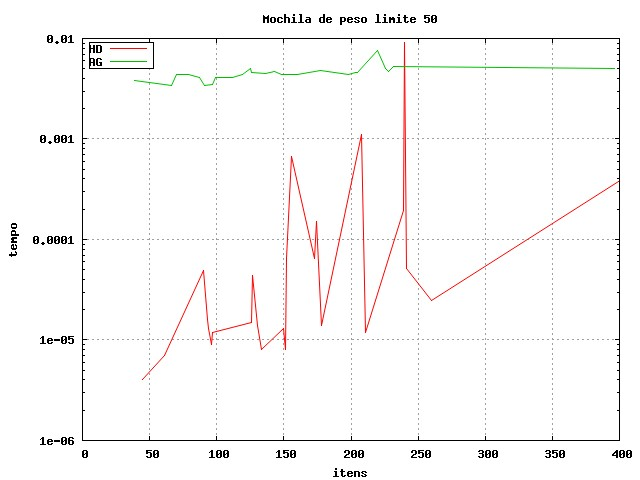
\includegraphics[scale=0.4]{images/w50.jpg}
	\caption{Gráfico comparativo dos tempos de execução dos quatro métodos: força bruta(FB), branch-and-bound(BB), programação dinâmica(PD) e algoritmos genéticos(AG), para mochilas com capacidade 50.}
	\label{fig:w50}
\end{figure}

Na figura~\ref{fig:w100}, podemos ver que o algoritmo genético obtêm tempo melhor que o algoritmo que utiliza \textit{branch-and-bound} a partir de 55 itens, mas que ainda se mantêm distante do tempo do algoritmo que utiliza programação dinâmica. Para esse tipo de mochila, o algoritmo genético gerou, em 24\% dos casos de teste, as soluções ótimas.

\begin{figure}[htp]
	\centering
	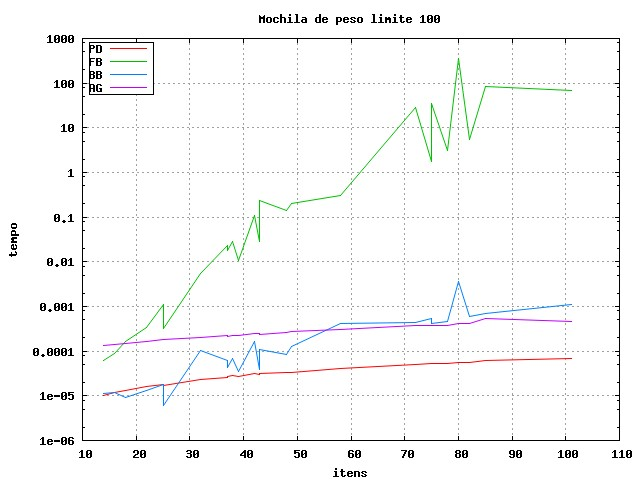
\includegraphics[scale=0.4]{images/w100.jpg}
	\caption{Gráfico comparativo dos tempos de execução dos quatro métodos: força bruta(FB), branch-and-bound(BB), programação dinâmica(PD) e algoritmos genéticos(AG), para mochilas com capacidade 100.}
	\label{fig:w100}
\end{figure}

Na figura~\ref{fig:w150}, em comparação com a figura~\ref{fig:w100}, podemos ver como o tempo do algoritmo genético começa a se aproximar do tempo do algoritmo que utiliza programação distribuida. O algoritmo genético gerou apenas uma solução ótima para esses casos de teste.

\begin{figure}[htp]
	\centering
	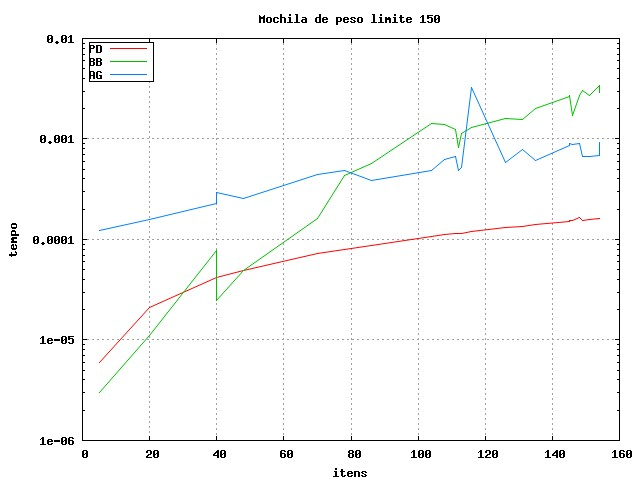
\includegraphics[scale=0.4]{images/w150.jpg}
	\caption{Gráfico comparativo dos tempos de execução dos três métodos mais rápidos: branch-and-bound(BB), programação dinâmica(PD) e algoritmos genéticos(AG), para mochilas com capacidade 150.}
	\label{fig:w150}
\end{figure}

Na figura~\ref{fig:w500}, podemos ver uma aproximação dos tempos de execução do algoritmo genético com o algoritmo que utiliza programação dinâmica. O algoritmo que utiliza \textit{branch-and-bound} é mais rápido para esse tipo de mochila quando o número de itens não ultrapassa 150. A partir desse ponto, o algoritmo se torna uma mais lento que os outros dois. Para esses casos de teste o algoritmo genético não gerou nenhuma solução ótima.

\begin{figure}[htp]
	\centering
	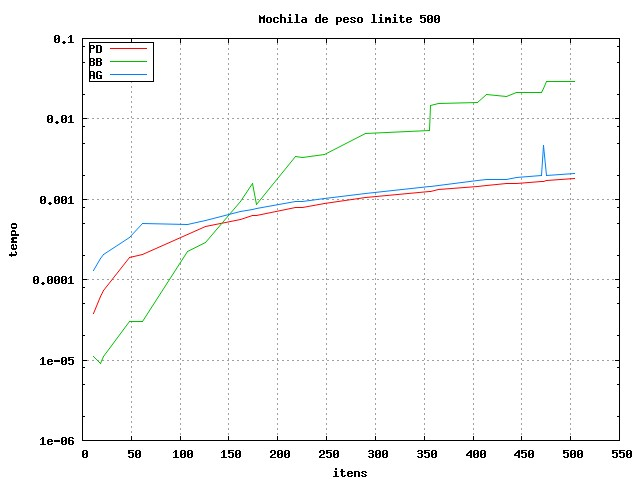
\includegraphics[scale=0.4]{images/w500.jpg}
	\caption{Gráfico comparativo dos tempos de execução dos três métodos mais rápidos: branch-and-bound(BB), programação dinâmica(PD) e algoritmos genéticos(AG), para mochilas com capacidade 500.}
	\label{fig:w500}
\end{figure}

Como podemos ver na figura~\ref{fig:w1000}, o algoritmo genético fica mais rápido que o algoritmo que utiliza programação dinâmica para quantidades grandes de itens e limites da mochila altos. o algoritmo que utiliza \textit{branch-and-bound} apresenta o mesmo comportamento que nas figuras anteriores, começa sendo rápido para uma quantidade pequena de itens e, a partir de um certo número de itens, tem o tempo maior que os outros dois algoritmos. Assim como nos casos de teste da mochila anterior, o algoritmo genético não encontrou nenhuma solução ótima.

\begin{figure}[htp]
	\centering
	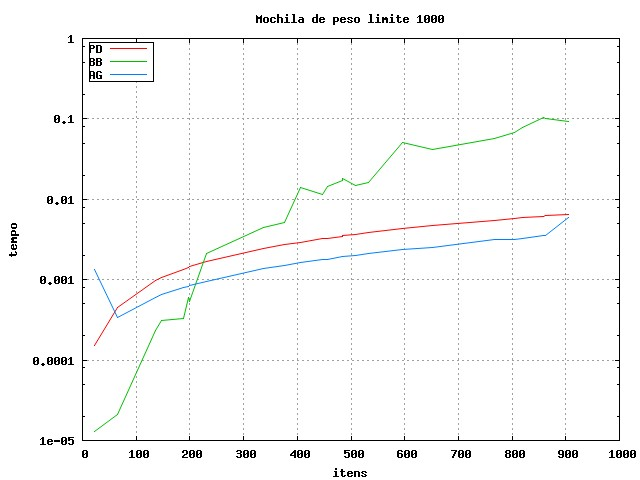
\includegraphics[scale=0.4]{images/w1000.jpg}
	\caption{Gráfico comparativo dos tempos de execução dos três métodos mais rápidos: branch-and-bound(BB), programação dinâmica(PD) e algoritmos genéticos(AG), para mochilas com capacidade 1000.}
	\label{fig:w1000}
\end{figure}

\newpage

\section{Mochila Compartimentada}
\subsection{Mochila Compartimentada usando Heurística da Decomposição}
A implementação deste algoritmo foi feita utilizando $K - 1$ chamadas ao algoritmo 1, que utiliza força bruta, uma para cada agrupamento de itens, para que fossem escolhidas os melhores compartimentos de cada agrupamento. Com esses compartimentos armazenados em um vetor, foi feita uma última chamada ao mesmo algoritmo, para que fossem escolhidos os compartimentos que entrariam na mochila.

\subsection{Mochila Compartimentada usando Algoritmo Genético}
Esse algoritmo genético é uma modificação do algoritmo da seção~\ref{cap4:gen}. Os pesos de cada compartimento são verificados e, se ultrapassarem o limite do compartimento, também sofrem penalidades. Com exeção dessa nova restrição, o algoritmo permanece o mesmo.


\begin{algorithm}
\caption{Avalie\_Compartimentada} %titulo do algoritmo
\scriptsize
\begin{algorithmic}[1]

  \STATE $maxprofit = 1$

  \FOR{$i = 0 \ at\acute{e} \ population\_size$}
    \STATE $profitFitness[i] = 0$
    \STATE $weightFitness[i] = 0$

    \WHILE{$!(stop) \&\& (j <= csize)$}

      \IF{$cur[i].cromo[j]$}

				\IF{$cur[i].type[itens[j].k] == 0$}
					\STATE $cur[i].type[itens[j].k] = 1$
					\STATE $cur[i].weight += S + itens[j].w$
					\STATE $cur[i].stype[itens[j].k] += S + itens[j].w$
					\STATE $cur[i].profit += (itens[j].p - c[itens[j].k])$
				\ELSE
					\STATE $cur[i].profit += itens[j].p$
					\STATE $cur[i].weight += itens[j].w$
					\STATE $cur[i].stype[itens[j].k] += itens[j].w$
				\ENDIF

				\IF{$cur[i].stype[itens[j].k] > L[itens[j].k]$}
					\STATE $cur[i].profit = 0$
					\STATE $cur[i].weight = 1$
					\STATE $stop = 0$
				\ENDIF
			\ENDIF
			\STATE $j++$
    \ENDWHILE

    \IF{$weight[i] > W$}
      \STATE $weight[i] = -(weight[i] - W)$
		\ENDIF

    \IF{$maxprofit < profit[i]$}
      \STATE $maxprofit = profit[i]$
		\ENDIF
  \ENDFOR

  \FOR{$i = 0 \ at\acute{e} population\_size$}
    \STATE $profitFitness[i] = 1 - (profit[i] / maxprofit) / psize$
    \STATE $weightFitness[i] = (weight[i] / W) / psize$
  \ENDFOR

\end{algorithmic}
\end{algorithm}


\subsection{Comparações relevantes}
As simulações computacionais foram feitas em um computador com processador AMD Sempron(tm) Processor 2800 e 1GB de memória. Foram feitas duas mochilas de pesos 50 e 100, com 25 casos de teste para cada mochila. Os valores para o número de itens e para seus pesos e benefícios foram gerados aleatoriamente.

\begin{itemize}
	\item Número de gerações: 50.
	\item Tamanho da população: 30.
	\item Taxa de \textit{cross-over}: 60\%.
	\item Taxa de mutação: 5\%.
\end{itemize}

Na figura~\ref{fig:com_w50}, vemos que o algoritmo genético não é tão eficiente para mochilas pequenas, uma vez que para verificar se uma configuração da mochila é válida o tempo gasto é grande. O algoritmo genético para ela encontrou a solução ótima em apenas um caso de teste, com razão de aproximação próxima a 1 em 44\% dos casos e, nos demais, com razão de aproximação próxima a 2. 

\begin{figure}[htp]
	\centering
	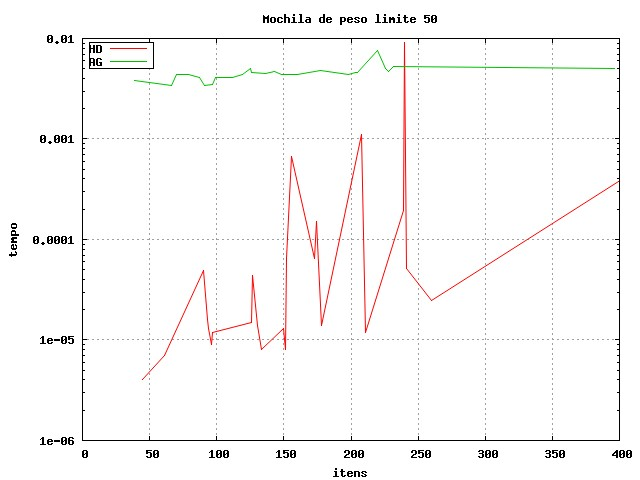
\includegraphics[scale=0.4]{images/com_w50.jpg}
	\caption{Gráfico comparativo dos tempos de execução dos dois métodos: heurística da decomposição(HD) e algoritmos genéticos(AG), para mochilas com capacidade 50.}
	\label{fig:com_w50}
\end{figure}

Com o aumento no número de itens e no limite da mochila, o algoritmo genético permanece com o mesmo tempo dos teste com a mochila de peso limite igual a 50, como podemos ver na figura~\ref{fig:com_w100}. Ao mesmo tempo, podemos ver o aumento no tempo de execução do algoritmo que utiliza a heurística da decomposição. Assim como na mochila anterior, o algoritmo genético encontrou a solução ótima em apenas um caso e, em 52\% dos casos, encontrou uma solução com razão de aproximação próxima a 2.

\begin{figure}[htp]
	\centering
	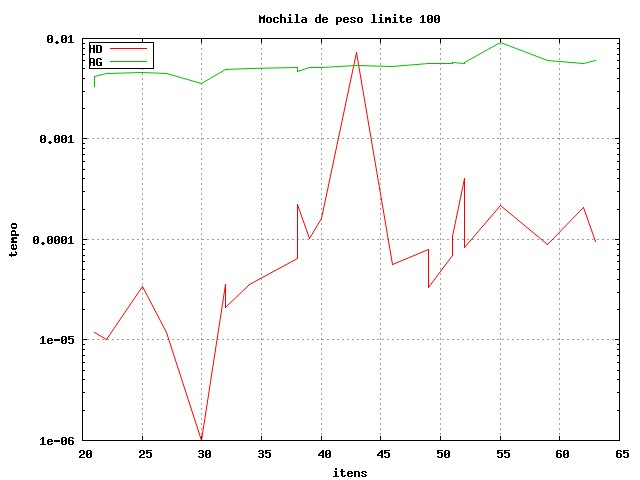
\includegraphics[scale=0.4]{images/com_w100.jpg}
	\caption{Gráfico comparativo dos tempos de execução dos dois métodos: heurística da decomposição(HD) e algoritmos genéticos(AG), para mochilas com capacidade 100.}
	\label{fig:com_w100}
\end{figure}

%Na figura~\ref{fig:com_w150}, podemos ver que, para alguns casos, o tempo de execução do algoritmo genético é melhor do que o tempo do algoritmo que utiliza a heurística da decomposição. Porém, o algoritmo genético não gerou nenhuma solução ótima para esse tipo de mochila.

%\begin{figure}[htp]
%	\centering
%	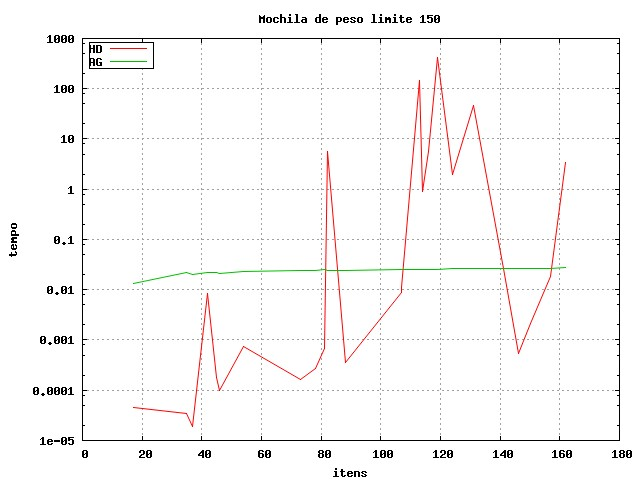
\includegraphics[scale=0.4]{images/com_w150.jpg}
%	\caption{Gráfico comparativo dos tempos de execução dos dois métodos: heurística da decomposição(HD) e algoritmos genéticos(AG), para mochilas com capacidade 150.}
%	\label{fig:com_w150}
%\end{figure}
